\documentclass[xcolor=pdftex,divnames,table]{beamer}%Creaci�n del tipo de documento, en este caso ser� una presentaci�n.Y permite
\usepackage[spanish]{babel}
\usepackage[latin1]{inputenc}
\usepackage{hyperref}
\usetheme{CambridgeUS}%El tema Warsaw para el esqueleto de futuras presentaciones.
\usepackage{color,xcolor}
\usepackage{booktabs}
\usepackage{ragged2e}
\usepackage{graphicx}
\usepackage{float}
\usepackage{listings}%Para c�digo bonito
\title{Taller b�sico de \LaTeX}%%Espacio para el t�tulo.
\author{Ponente: V�ctor Hugo V�zquez Montoya}
\institute{\href{mailto:victor.hugovz@comunidad.unam.mx}{victor.hugovz@comunidad.unam.mx}}
\date{FLISOL 2019}

\begin{document}
\frame{\titlepage}
\frame{\tableofcontents}
\section{�Qu� es \LaTeX\, y porqu� se considera software libre?}

\begin{frame}%%Inicio de Bloque
\justify
\begin{itemize}%PRIMER BLOQUE DE COMANDOSCreaci�n de la lista numeradas
\item Es un sistema de alta calidad tipogr�fica con 
caracter�sticas dise�adas para la producci�n de documentaci�n cient�fica
\item Esta disponible como software libre bajo los t�rminos de la licencia p�blica del proyecto \LaTeX
\item �\LaTeX\, no es un procesador de textos!
\end{itemize}%Finaliza la lista numerada
\end{frame}%Fin del Bloque y primera secci�n%
\section{Objetivo}
\begin{frame}
\justify
\LaTeX\, anima a los autores a no preocuparse demasiado por la apariencia de sus documentos, sino a concentrarse en 
\textit{obtener el contenido correcto}
\end{frame}
\section{Breve historia}
\begin{frame}
\begin{center}
 \LaTeX\, en un principio es un lenguaje de macros creado en 1982 por Leslie Lamport para facilitar en aquel momento la 
composici�n de textos con el compilador \TeX\, el cual hab�a aparecido en 1978 de la mano de Donald Ervin Knuth en la Universidad 
de Staford
\end{center}
 \begin{columns}
  \column{2in}
  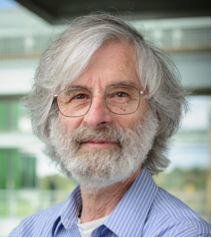
\includegraphics{lamport.png}
  \newline 
  \column{2in}
  \includegraphics[scale=0.47]{Donald.jpeg}
 \end{columns}
\end{frame}
\section{�C�mo obtengo \LaTeX?}
\begin{frame}
\begin{itemize}
 \item \LaTeX\, es distribuido a trav�s de los servidores CTAN, viene como parte de muchas distribuciones \TeX\, que son 
f�cilmente 
instalables y usables proveidas por el Grupo de Usuarios \TeX\, (TUG).
\end{itemize}
\end{frame}
\begin{frame}
\begin{columns} 
\column{2in}
\begin{itemize}
 \item \textbf{Linux.} Compruebe su fuente de software de distribuciones de Linux para una distribuci�n \TeX\, incluyendo \LaTeX.
\item \textbf{MAC OS.} La distribuci�n de Mac\TeX, contiene todo lo que necesitas, incluyendo un completo sistema \TeX\, con 
editores para escribir documentos.
\end{itemize}

\column{2in}
\begin{itemize}
\item \textbf{Windows.} Las distribuciones MiK\TeX\, contienen un sistema
completo y editores para escribir documentos.
\item \textbf{Nube.} Servicios en l�nea de \LaTeX\, como Papeeria, Overleaf, Datazar y \LaTeX\, base ofrecen la 
posibilidad de editar, ver y descargar archivos \TeX\, y PDF resultantes.
\end{itemize}
\end{columns}
\end{frame}
\section{�Se usa fuera del modo matem�tico?}
\begin{frame}
 \justify
 Actualmente, \LaTeX\, es un producto muy evolucionado y respecto a su espectacular auge ha contribuido el que sea un producto 
gratuito, de gran fexibilidad que naci� para adaptarse a las evoluciones matem�ticas. Es utilizado en el \texttt{plan 
profesional} por muchas empresas editoriales de cualquier �mbito.
\begin{center}
 
\includegraphics[scale=0.5]{latexproject.png}
\end{center}
\end{frame}

\section{�C�mo funciona \LaTeX?}
\begin{frame}
\textbf{Ingredientes}
\begin{itemize}
 \item Compilador de \LaTeX/PDF\LaTeX
 \item Editor de textos ASCII
 \item Un visualizador como Adobe Acrobat Reader
\end{itemize}
\begin{center}
 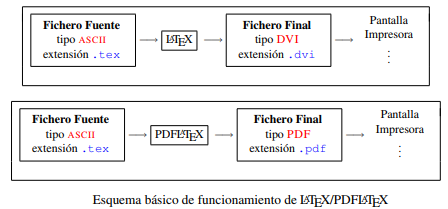
\includegraphics[scale=0.4]{funcionamiento.png}
 \end{center}
\end{frame}
\section{Previo a escribir c�digo\ldots}
\begin{frame}
\frametitle{Caracteres reservados}
 \begin{table}
  \begin{tabular}{c|c|}
   \textbf{Caracter} & \textbf{C�mo lo debo teclear en c�digo \TeX}\\ \hline
   \$ & \textbackslash{}\$ \\ \hline
   \& & \textbackslash{}\& \\ \hline
   \# & \textbackslash{}\# \\ \hline
   \% & \textbackslash{}\% \\ \hline
   \_ & \textbackslash{}\_ \\ \hline
   \textbackslash & \textbackslash{textbackslash}\\ \hline
   \{ & \textbackslash{}\{ \\ \hline
   \} & \textbackslash{}\} \\ \hline
  \end{tabular}
\caption{Algunos caracteres especiales en \LaTeX}
 \end{table}
\end{frame}
\section{Contenido breve del taller}
\begin{frame}
\frametitle{Temas a tratar:}
 \begin{enumerate}
  \item Estructura de un documento en \LaTeX
  \item Algunos entornos matem�ticos
  \item Tablas y figuras
  \item Bibliograf�as artesanales
 \end{enumerate}
\end{frame}
\section{Referencias}
\begin{frame}{Bibliograf�a}
\begin{thebibliography}{9}
\bibitem{texbook}
Donald E. Knuth (1986) \emph{The \TeX{} Book}, Addison-Wesley Professional.

\bibitem{lamport94}
Leslie Lamport (1994) \emph{\LaTeX: a document preparation system}, Addison
Wesley, Massachusetts, 2nd ed.
\end{thebibliography}
\end{frame}
\end{document}%Fin del documento/presentaci�n